\clearpage{}
\section{Explain the principles of fault tree analysis and cut-set
computation. Explain the principles of trade-off analysis with weighted
comparisons. Describe cost-benefit analysis based on return on
investment and payback period. Define the notion of quality model and
describe an example.}

\subsection{Fault tree analysis}

Fault tree analysis is a method that helps us to examine a design and
look for fault that might lead to failure.

\begin{figure}[!ht]
    \centering
    \begin{minipage}{\linewidth}
        \begin{minipage}{0.45\linewidth}
            \centering
            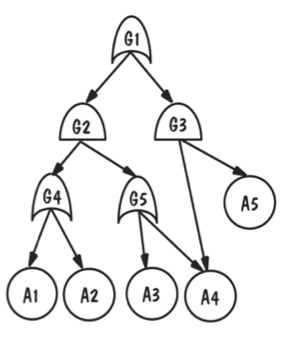
\includegraphics[width=0.8\linewidth]{fault_tree_analysis.png}
        \end{minipage}
        \begin{minipage}{0.45\linewidth}
            Root = failure

            Leaves = faults, events

            Nodes = logic gates (AND/OR)

            Edges = caused-by
        \end{minipage}
    \end{minipage}
\end{figure}

Building fault tree:
\begin{enumerate}
    \item Identify possible failures
    \item For each failure, build the fault tree trace backwards through the design
\end{enumerate}

\subsection{Cut-set computation}

The cut-set is the minimal set of events (faults) that can cause a failure. 

\begin{figure}[!ht]
    \begin{minipage}{\linewidth}
        \begin{minipage}{0.45\linewidth}
            \centering
            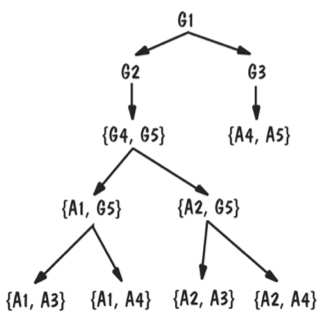
\includegraphics[width=0.8\linewidth]{cut_set_computation.png}
        \end{minipage}
        \begin{minipage}{0.45\linewidth}
            Nodes = sets of nodes of the fault tree

            Root = \{ root of fault tree \}

            Leaves = sets of leaves of the fault tree
            = cut-sets
        \end{minipage}
    \end{minipage}
\end{figure}

Building cut-set tree:
\begin{enumerate}
    \item Assign the top node of the cut-set tree to match the logic gate at the top of the fault
tree
    \item Working from the top down, expand the cut-set tree as follows:
    \begin{itemize}
        \item Expand an or-gate node to have two children, one for each or-gate child
        \item Expand an and-gate node to hate a child composition node listing both of the and-gate children
        \item Expand a composition node by propagating the node to its children, but expanding one of the gates listed the node
    \end{itemize}
    \item Continue until all leaf nodes are basic events or composition nodes of basic events
\end{enumerate}

\subsection{Trade-off analysis with weighted comparisons}

We have often several alternative designs to consider. To make a good choice we need a
measurement-based method for comparing design alternatives.
\textbf{Weighted comparison} is a example of measurement method.

\begin{figure}[!ht]
    \centering
    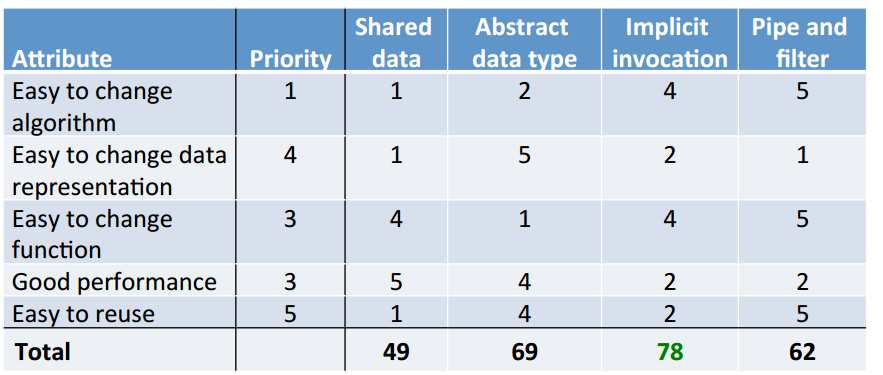
\includegraphics[width=0.6\linewidth]{trade_off_analysis.png}
\end{figure}

All the designs are on X-axis, and judgment criterions are on Y-axis. 
Give a score for each (subjective values based on past projects), and
select the solution with the best global score.

\subsection{Cost-benefit analysis}

Evaluation of the design based on business aspects and economical value
of the product rather than design quality: benefits vs.\ cost.

\begin{figure}[!ht]
    \centering
    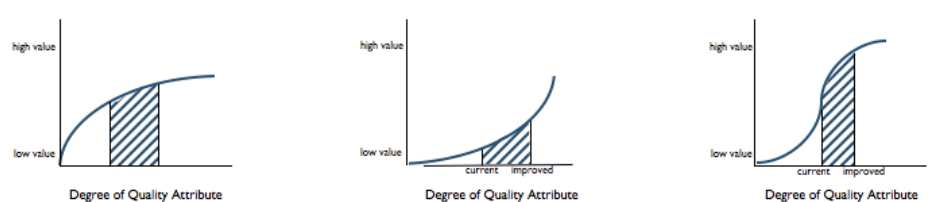
\includegraphics[width=\linewidth]{cost_benefit_analysis.png}
\end{figure}

Value is not linearly dependant of quality\ldots

$\Rightarrow$ You have to find the best compromise to increase ROI
or the minimal payback period (number years before winning money)
$$ \text{ROI} = \frac{\text{Total benefits}}{\text{Total cost}}$$
$$\text{Payback period} = \frac{\text{Benefits}}{\text{years}} \times
\frac{1}{\text{benefits}}$$

\subsection{Quality model}

Looking for the desirable attributes of a product (e.g.\ document, file,
system\ldots).
The \textbf{product quality model} makes hierarchical nomenclature of product quality characteristics. 
\newline

\begin{figure}[!ht]
    \centering
    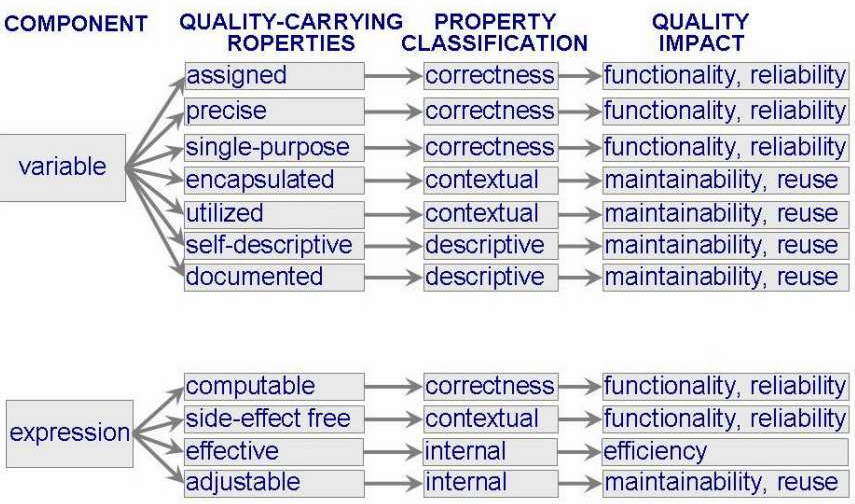
\includegraphics[width=0.8\linewidth]{dromey_quality_model.png}
    \caption{Dromey Quality Model: Example}
\end{figure}

In the example above, you see that different components (variable,
expression) are associated to some quality (documented,
encapsulated\ldots) that are classified and associated to a quality
impact. 

Baseline and targets:
\begin{itemize}
    \item Measure quality attributes relative to baseline (typical result)
    \item Require quality attribute relative to target (minimal acceptable result)
\end{itemize}
